%%%%%%%%%%%%%%%%%%%%%%%%%%%%%%%%%%%%%%%%%
% a0poster Portrait Poster
% LaTeX Template
% with University Copenhagen logo
% Version 1.0 (22/06/13)
%
% Based on:
% The a0poster class was created by:
% Gerlinde Kettl and Matthias Weiser (tex@kettl.de)
%
% This template has been downloaded from:
% http://www.LaTeXTemplates.com
%
%%%%%%%%%%%%%%%%%%%%%%%%%%%%%%%%%%%%%%%%%
% cd /disks/PROJECT/Mickael/COMMUNICATION/IGES2015/;
% pdflatex PosterIGES.tex; bibtex PosterIGES; pdflatex PosterIGES.tex; pdflatex PosterIGES.tex;
% evince PosterIGES.pdf &

% \color{ku}
% \color{SaddleBrown}
% \color{DarkSlateGray}

%----------------------------------------------------------------------------------------
%    PACKAGES AND OTHER DOCUMENT CONFIGURATIONS
%----------------------------------------------------------------------------------------

\documentclass[a0,portrait]{a0poster}
\pdfpageattr{/Group << /S /Transparency /I true /CS /DeviceRGB>>}
\usepackage[utf8]{inputenc}

\usepackage{multicol} % This is so we can have multiple columns of text side-by-side
\usepackage[left=3cm,right=3cm,top=3.5cm,bottom=1cm]{geometry}
\usepackage[usenames, dvipsnames, svgnames, x11names, hyperref, RGB]{xcolor} % Specify colors by their 'svgnames', for a full list of all colors available see here: http://www.latextemplates.com/svgnames-colors

% \usepackage{times} % Use the times font
%\usepackage{palatino} % Uncomment to use the Palatino font

\usepackage{graphicx} % Required for including images
\graphicspath{{figures/}} % Location of the graphics files
\usepackage{booktabs} % Top and bottom rules for table
\usepackage[format=plain, font=large, labelfont=bf, hang]{caption} % Required for specifying captions to tables and figures
\usepackage{amsfonts, amsmath, amsthm, amssymb} % For math fonts, symbols and environments
\usepackage{wrapfig} % Allows wrapping text around tables and figures
\definecolor{ku}{RGB}{144,26,30}
\definecolor{ku-yellow}{RGB}{255,249,25}

\usepackage{helvet}
\renewcommand{\familydefault}{\sfdefault}
\usepackage{courier}

\usepackage{multirow}
\usepackage{arydshln}
\usepackage{indentfirst}

\definecolor{dodgerblue}{RGB}{30,144,255}
\definecolor{springgreen3}{RGB}{0,139,69}
\definecolor{firebrick2}{RGB}{238,44,44}
\definecolor{maroon2}{RGB}{238,48,167}
\definecolor{goldenrod2}{RGB}{238,180,34}
\definecolor{deepskyblue}{RGB}{0,191,255}

\newcommand\bref[2]{\hyperref[#1]{#2~\ref*{#1}}}
\newcommand\cmd[1]{{\texttt{\color{black}\textbf{#1}}}}
\newcommand\cmdb[1]{{\color{dodgerblue}\textbf{#1}}}
\newcommand\cmdr[1]{{\color{firebrick2}\textbf{#1}}}
\newcommand\cmdg[1]{{\color{springgreen3}\textbf{#1}}}
\newcommand\cmdy[1]{{\color{goldenrod2}\textbf{#1}}}

\usepackage[square, authoryear]{natbib}

\usepackage[colorlinks=true,
    linkcolor=firebrick2,
    urlcolor=maroon2,
    citecolor=dodgerblue,
    filecolor=goldenrod2,
    menucolor=dodgerblue,
    pdftex=true,
    bookmarks=true,
    bookmarksopen=true,
    hyperfootnotes=true,
    pdfauthor={Mickaël Canouil},
    pdfcreator={Mickaël Canouil}]{hyperref}
\renewcommand{\thefootnote}{\textcolor{springgreen3}{\arabic{footnote}}}

\usepackage[english]{babel}
\selectlanguage{english}

\newcommand{\superscript}[1]{\ensuremath{^{\textrm{#1}}}}

\renewcommand{\baselinestretch}{1.15}
\setlength{\tabcolsep}{20pt}

\setlength{\columnsep}{100pt}
\setlength{\columnseprule}{5pt}

\usepackage{eso-pic}
\usepackage{transparent}



\begin{document}
\AddToShipoutPicture*{\AtPageLowerLeft{\transparent{0.20}\includegraphics[width=\paperwidth,height=\paperheight]{figures/BG01_A0.png}}}
\Large
%----------------------------------------------------------------------------------------
%    POSTER HEADER
%----------------------------------------------------------------------------------------
% The header is divided into two boxes:
% The first is 75% wide and houses the title, subtitle, names, university/organization and contact information
% The second is 25% wide and houses a logo for your university/organization or a photo of you
% The widths of these boxes can be easily edited to accommodate your content as you see fit

\begin{minipage}[t]{0.60\linewidth}
\flushleft
{\Huge \textcolor{ku}{\textbf{\mbox{Application} of \mbox{Joint} \mbox{Models} in \mbox{Genetic} \mbox{Association} \mbox{Studies}}}}\\ % Title
\vspace{1cm}
{\large \textbf{Ghislain Rocheleau\superscript{1,2,3}, Mickaël Canouil\superscript{1,2,3}, Loïc Yengo\superscript{2,3}, Philippe Froguel\superscript{1,2,3,4}}\\[0.5cm] % Author(s)
\textcolor{DarkSlateGray}{
\superscript{1}Lille 2 University, Lille, France\\
\superscript{2}UMR 8199 - Pasteur Institute, Lille, France\\
\superscript{3}FR 3508 - European Genomic Institute for Diabetes, Lille, France\\
\superscript{4}Department of Genomics of Common Disease, Imperial College London, London, United Kingdom\\
}}
\end{minipage}
%
\begin{minipage}[t]{0.40\linewidth}
\flushright
\textcolor{DarkSlateGray}{
{\large \textbf{Contact informations:}\\
CNRS UMR8199 - Institut de Biologie de Lille\\
1 Rue du Professeur Calmette\\
BP 245\\
F-59019 LILLE CEDEX\\[1.5cm]
+33(0)3-20-87-11-07\\[0.20cm]
\texttt{ghislain.rocheleau@cnrs.fr}}
}
\end{minipage}

% \vspace{1cm} % A bit of extra whitespace between the header and poster content


%----------------------------------------------------------------------------------------

% \begin{multicols}{2} % This is how many columns your poster will be broken into, a portrait poster is generally split into 2 columns

%----------------------------------------------------------------------------------------
%    ABSTRACT
%----------------------------------------------------------------------------------------
% \begin{abstract}
% \end{abstract}


%----------------------------------------------------------------------------------------
%    INTRODUCTION
%----------------------------------------------------------------------------------------
\color{SaddleBrown}
\section*{Introduction}
\par{To optimize use of existing phenotypic data, we propose a joint model \citep{tsiatis2004} approach aimed at identifying genetic markers
simultaneously associated to temporal trajectories of a trait and an event outcome.
Standard formulation of the joint model involves two components: a longitudinal component and a time-to-event component.
We illustrate the application of the joint model approach in genetic epidemiology by exploiting the strong link
between temporal variation of blood glucose levels (FG) and onset of type 2 diabetes (T2D).
Using genotypes assayed with the Metabochip DNA arrays (Illumina) from 4,500 subjects recruited
in the French cohort D.E.S.I.R. (Donn\'{e}es \'{E}pid\'{e}miologiques sur le Syndrome d’Insulino-R\'{e}sistance),
we reexamine previous GWAS findings for some confirmed glycaemia and T2D loci.}


\color{DarkSlateGray}
\begin{multicols}{2}
%----------------------------------------------------------------------------------------
%    MATERIALS AND METHODS
%----------------------------------------------------------------------------------------
\section*{Methods}
\begin{center}
    \fbox{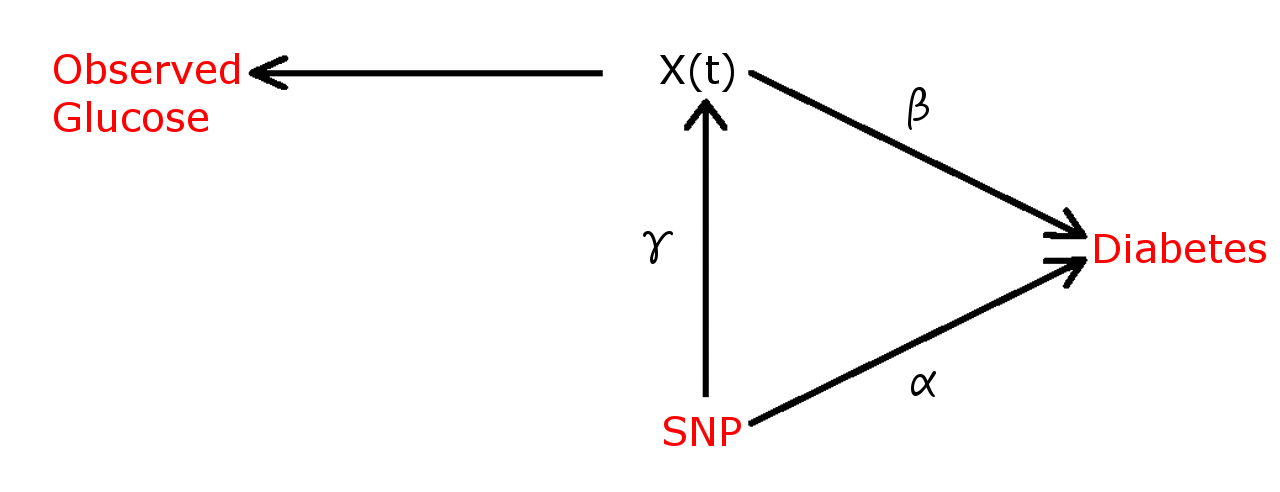
\includegraphics[width=0.8\linewidth]{jointModel.png}}
    \captionof{figure}{\color{springgreen3} Causal diagram for joint modeling (adapted from \citet{ibrahim2010}).}
    \label{Fig1}
\end{center}
\vspace{1cm}
\par{The longitudinal component typically consists of a linear mixed model:}

\begin{minipage}[t]{0.475\columnwidth}
\vspace{-1cm}%
\hspace{-10cm}
{\color{springgreen3}%
\begin{eqnarray}Y_{ij}=X_{ij}+\epsilon_{ij}\nonumber\label{Eq1}\end{eqnarray}
\begin{eqnarray}X_{ij}=\theta_{0i}+\theta_{1i}\times t_{ij}+\gamma \times SNP_i\nonumber\label{Eq2}\end{eqnarray}
\begin{eqnarray}\boldsymbol\theta \sim \mathcal{N}_2(\boldsymbol\mu, \boldsymbol\Sigma)\nonumber\label{Eq3}\end{eqnarray}
\begin{eqnarray}\epsilon_{ij} \sim \mathcal{N}(0, \sigma^2)\nonumber\label{Eq4}\end{eqnarray}
}%
\vspace{-1.5cm}
\end{minipage}%
\hfill\vline\hfill
\begin{minipage}[t]{0.475\columnwidth}%
\vspace{0.8cm}%
\par{{\color{springgreen3}$Y_{ij}$}: observed value;}
\vspace{1.75cm}%
\par{{\color{springgreen3}$X_{ij}$}: true (unobserved) value of the longitudinal variable;}
\vspace{1.75cm}%
\par{{\color{springgreen3}$\gamma$}: SNP effect on the trajectory function (\bref{Fig1}{Figure}).}
\end{minipage}
\vspace{1cm}%
\par{Using the Cox model for the time-to-event (survival) component, we define:}
{\color{springgreen3}\begin{eqnarray}\lambda_i(t)=\lambda_0(t) exp(\beta X_i(t)+\alpha SNP_i)\nonumber\label{Eq5}\end{eqnarray}}
\begin{minipage}[t]{0.475\columnwidth}
\vspace{0.10cm}%
\par{{\color{springgreen3}$\lambda_i(t)$}: hazard function at time {\color{springgreen3}$t$}}
\vspace{1.85cm}%
\par{{\color{springgreen3}$\lambda_0(t)$}: (unspecified) baseline hazard function.}
\end{minipage}%
\hfill\vline\hfill
\begin{minipage}[t]{0.475\columnwidth}%
\vspace{0.10cm}%
\par{{\color{springgreen3}$\alpha$}: SNP effect on time-to-event (\bref{Fig1}{Figure}).}
\par{{\color{springgreen3}$\beta$}: association between the trajectory function and time-to-event (\bref{Fig1}{Figure}).}
\end{minipage}


%----------------------------------------------------------------------------------------
%    RESULTS
%----------------------------------------------------------------------------------------
\section*{Results}
\vspace{-1cm}
\par{As expected, we confirm some findings from GWAS,
especially the strong association between FG and some SNP ({\color{springgreen3}$\gamma \neq 0$}) in G6PC2, GCKR
and MTNR1B genes (\bref{Tab1}{Table}).}
\columnbreak
\begin{center}
    \begin{tabular}{rccc}
        \hline
        & $\gamma$ & $\alpha$ & $\beta$ \\
        \hline
        rs7903146 (TCF7L2) & \textcolor{dodgerblue}{0.02465} & 0.2204 & \textcolor{firebrick2}{3.477} \\
        rs3802177 (SLC30A8) & \textcolor{dodgerblue}{0.038} & 0.01066 & \textcolor{firebrick2}{3.542} \\
        rs10278336 (GCK) & \textcolor{dodgerblue}{0.0383} & 0.09214 & \textcolor{firebrick2}{3.527} \\
        rs560887 (G6PC2) & \textcolor{firebrick2}{0.09504} & \textcolor{dodgerblue}{-0.3237} & \textcolor{firebrick2}{3.568} \\
        rs780094 (GCKR) & \textcolor{firebrick2}{0.06271} & -0.09694 & \textcolor{firebrick2}{3.568} \\
        rs10830963 (MTNR1B) & \textcolor{firebrick2}{0.0959} & \textcolor{dodgerblue}{-0.3868} & \textcolor{firebrick2}{3.611} \\
        rs11717195 (ADCY5) & \textcolor{dodgerblue}{0.02581} & -0.1202 & \textcolor{firebrick2}{3.554} \\
        \hline
    \end{tabular}
    \captionof{table}{\color{springgreen3} Parameter estimates from R package \cmd{JM} \citep{rizopoulos_jm_2010} applied to a selection of SNPs.
    In \textcolor{dodgerblue}{blue}: $\textrm{p-value}<0.05$, in \textcolor{firebrick2}{red}: $\textrm{p-value}<5\times 10^{-8}$.}
    \label{Tab1}
\end{center}
\vspace{1cm}
\par{The association between FG and T2D risk is highly significant ({\color{springgreen3}$p<10^{-50}$}) as a result of the T2D diagnosttic ({\color{springgreen3}$FG>7mM/L$}).}


%----------------------------------------------------------------------------------------
%    POWER ESTIMATION
%----------------------------------------------------------------------------------------
\section*{Power estimation}
\vspace{-2cm}
\begin{minipage}[t]{0.475\columnwidth}
\vspace{1.5cm}
\begin{center}
    \begin{tabular}{c:c:c:c}
    \hline
        $f$ & $\alpha$ & $\gamma$ & Power \\
    \hline
        \multirow{9}{*}{0.30} & \multirow{3}{*}{0.10} & 0.05 & 0.41 \\
            &  & 0.06 & 0.49 \\
            &  & 0.07 & 0.58 \\
            \hdashline
            & \multirow{3}{*}{0.20} & 0.05 & 0.65 \\
            &  & 0.06 & 0.73 \\
            &  & 0.07 & 0.80 \\
            \hdashline
            & \multirow{3}{*}{0.30} & 0.05 & 0.85 \\
            &  & 0.06 & 0.89 \\
            &  & 0.07 & 0.93 \\
    \hline
    \end{tabular}
    \captionof{table}{\color{springgreen3} Power estimation from \mbox{formula} derived in \citet{chen_sample_2011}.}
\end{center}
\end{minipage}%
\hfill\vline\hfill
\begin{minipage}[t]{0.475\columnwidth}%
\vspace{0cm}
\par{To detect global SNP effect \mbox{{\color{springgreen3}$\beta\gamma+\alpha$}}, we used equation:
{\color{springgreen3}
\begin{equation}\begin{split}
z_{\tilde{\beta}}=&\pm\sqrt{Df(1-f)(\beta\gamma+\alpha)^2} \\
&+z_{1-\tilde{\alpha}/2}\nonumber
\end{split}\end{equation}
}}
\par{{\color{springgreen3}$D$}: number of incident T2D cases;}
\par{{\color{springgreen3}$f$}: allele frequency.}
\vspace{1cm}
\par{Retrospective power estimations provided by the formula in \citet{chen_sample_2011} show consistent results with
our application for an estimated effect {\color{springgreen3}$\beta=3.5$} and {\color{springgreen3}$\tilde{\alpha}=0.05$}.}
\end{minipage}


%----------------------------------------------------------------------------------------
%    FUTURE RESEARCH
%----------------------------------------------------------------------------------------
\section*{Future research}
\vspace{-1cm}
\par{To the best of our knowledge, joint models have never been used in genetic association studies.
In particular, power estimation and effect of missing data remain to be studied in further details.}


\end{multicols}
%----------------------------------------------------------------------------------------
%    REFERENCES
%----------------------------------------------------------------------------------------
\color{SaddleBrown}
\normalsize
\bibliographystyle{apalike} % apalike
\bibliography{PosterIGES.bib} % Use the example bibliography file sample.bib
\begin{center}
    \vfill
    {
\includegraphics[height=6cm, keepaspectratio]{figures/logo_cnrs.pdf}
    \hspace{11cm} 
\includegraphics[height=6cm, keepaspectratio]{figures/UL2-WEB-2014.png}
    \hspace{8cm} 
\includegraphics[height=6cm, keepaspectratio]{figures/Institut-Pasteur-de-Lille.png}
    \hspace{11cm} 
\includegraphics[height=6cm, keepaspectratio]{figures/logo_egid.pdf}}
\end{center}


%----------------------------------------------------------------------------------------
\end{document}
